\section{Exercice 1 : Sur papier}
\subsection{Encodage du message $m=(1,1,0,1)$}
Pour encoder le message $m=(1,1,0,1)$, il faut multiplier ce message par la matrice génératrice $G$ donnée. La matrice génératrice $G$ est de la forme suivante :

\begin{equation}
 G=
\begin{pmatrix}
    1 & 0 & 0 & 0 & 0 & 1 & 1 \\
    0 & 1 & 0 & 0 & 1 & 0 & 1 \\
    0 & 0 & 1 & 0 & 1 & 1 & 0 \\
    0 & 0 & 0 & 1 & 1 & 1 & 1
   \end{pmatrix}
\end{equation}
Ainsi, en multipliant $m$ et $G$, nous obtenons le message $m_e$ suivant :
\begin{equation}
 m_e=m\times G=(1,1,0,1)\times
 \begin{pmatrix}
    1 & 0 & 0 & 0 & 0 & 1 & 1 \\
    0 & 1 & 0 & 0 & 1 & 0 & 1 \\
    0 & 0 & 1 & 0 & 1 & 1 & 0 \\
    0 & 0 & 0 & 1 & 1 & 1 & 1
   \end{pmatrix}
   =(1,1,0,1,0,0,1)
\end{equation}
\subsection{Vérification que $H$ est bien une matrice de contrôle}
Afin de vérifier si un mot de code reçu comporte des erreurs, il est possible multiplier ce dernier à une matrice de contrôle, $H$. Ici, la matrice $H$ est de la forme suivante :
\begin{equation}
 H=
 \begin{pmatrix}
  0 & 0 & 0 & 1 & 1 & 1 & 1 \\
  0 & 1 & 1 & 0 & 0 & 1 & 1 \\
  1 & 0 & 1 & 0 & 1 & 0 & 1
 \end{pmatrix}
\end{equation}
Afin de vérifier si cette matrice est bien un matrice de contrôle, nous allons vérifier cela avec notre mot encodé $m_e$.\\
Pour ce faire, nous allons multiplier $m_e$ et $H$. Nous obtiendrons alors deux résultats possibles :
\begin{itemize}
 \item Si le résultat $s$ est égal $(0,0,0)$, alors il n'y a aucune faute dans le mot code.
 \item Si le résultat $s$ n'est pas égal à $(0,0,0)$, alors le mot code comporte au moins une erreur. 
\end{itemize}
Ici, nous utiliserons un mot code que nous savons correct. Le résultat devra obligatoirement être égal à $(0,0,0)$ sauf si $H$ n'es pas une matrice de contrôle.
\begin{equation}
 s=H\times m_e=
  \begin{pmatrix}
  0 & 0 & 0 & 1 & 1 & 1 & 1 \\
  0 & 1 & 1 & 0 & 0 & 1 & 1 \\
  1 & 0 & 1 & 0 & 1 & 0 & 1
 \end{pmatrix}
 \times(1,1,0,1,0,0,1)=(0,0,0)
\end{equation}
Ainsi, nous savons que la matrice de contrôle $H$ est correcte.
\subsection{Vérification que $(1,1,1,1,1,1,1)$ est bien un de code}
Afin de vérifier si le message $c_2=(1,1,1,1,1,1,1)$ est bien un mot code, nous allons le multiplier avec la matrice de contrôle $H$ et observer le résultat :
\begin{equation}
 s_2=H\times c_2=
  \begin{pmatrix}
  0 & 0 & 0 & 1 & 1 & 1 & 1 \\
  0 & 1 & 1 & 0 & 0 & 1 & 1 \\
  1 & 0 & 1 & 0 & 1 & 0 & 1
 \end{pmatrix}
 \times(1,1,1,1,1,1,1)=(0,0,0)
\end{equation}
Le résultat $s_2$ étant bien égal à $(0,0,0)$, le mot encodé $c_2=(1,1,1,1,1,1,1)$ est bien un mot code. ce dernier, décodé est le mot $(1,1,1,1)$.
\subsection{Réception et correction du message $c'=(1,1,1,1,0,0,1)$}
Le mot de code reçu, $c'=(1,1,1,1,0,0,1)$, n'est pas un mot de code. pour le vérifier, nous allons multiplier $c'$ à la matrice $H$ de contrôle :
\begin{equation}
 s_3=H\times c'=
  \begin{pmatrix}
  0 & 0 & 0 & 1 & 1 & 1 & 1 \\
  0 & 1 & 1 & 0 & 0 & 1 & 1 \\
  1 & 0 & 1 & 0 & 1 & 0 & 1
 \end{pmatrix}
 \times(1,1,1,1,0,0,1)=(0,1,1)
\end{equation}
Comme nous pouvons le constater, le résultat $s_3=(0,1,1)$ est différent de $(0,0,0)$. Nous pouvons alors noter que $c'$ n'est pas un mot de code. \\
Cependant, nous savons qu'il ne comporte qu'une seule erreur. De plus, nous pouvons déduire grâce au résultat de $s_3$ connaître la position de ce bit erroné. En effet, en lisant le résultat $s_3$ en binaire (ici, $011=3$ en décimal), nous savons que l'erreur a été faite sur le troisième bit.\\
Nous obtenons alors le mot de code suivant :
\begin{equation}
 c'_2=(1,1,0,1,0,0,1)
\end{equation}
Afin de vérifier si cette correction est la bonne, nous allons vérifier que ce dernier est correct : 
\begin{equation}
 s_4=H\times c'_2=
  \begin{pmatrix}
  0 & 0 & 0 & 1 & 1 & 1 & 1 \\
  0 & 1 & 1 & 0 & 0 & 1 & 1 \\
  1 & 0 & 1 & 0 & 1 & 0 & 1
 \end{pmatrix}
 \times(1,1,0,1,0,0,1)=(0,0,0)
\end{equation}
Le résultat $s_4$ étant bien égal à $(0,0,0)$, nous pouvons conclure que $c'_2$ est bien un mot de code. Il peut être décodé en mot $m_{c'}=(1,1,0,1)$.


\section{Exercice 2: Le code}

Dans cette partie nous avons réaliser les différentes fonctions qui étaient demandées afin de faire une simulation sur un nombre aléatoire de mots (eux même générés aléatoirement) en fonction d'une probabilité que l'on passe en paramètre. Cette simulation va de 0.001 à 0.500 pour la valeur de la probabilité (noté p).\\
Le principe est simple:
\begin{itemize}
\item On choisit une valeur de p
\item On génère un mot aléatoirement
\item On l'encode
\item On génère du bruit sur ce mot
\item On le décode
\item On vérifie que le décodé est égale au mot d'origine
\item On recommence cette opération N fois pour la probabilité p donnée
\end{itemize}
Pour chacune des probabilités données, on effectue un grand nombre de fois l'algorithme précédent et on affiche dans la console les résultats suivants:
\begin{itemize}
\item La valeur de p
\item Le nombre de fois où le mot décodé est égale au mot d'origine
\item Le nombre de fois où le mot décodé n'est pas égale au mot d'origine
\end{itemize}
\newpage
On obtient alors des exemples de résultats suivants:
\begin{figure}
    \centering
    \begin{subfigure}[b]{0.3\textwidth}
        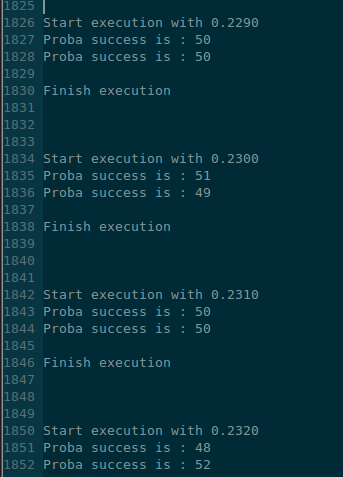
\includegraphics[width=\textwidth]{img/code.png}
        \label{fig:gull}
    \end{subfigure}
    ~ %add desired spacing between images, e. g. ~, \quad, \qquad, \hfill etc. 
      %(or a blank line to force the subfigure onto a new line)
    \begin{subfigure}[b]{0.3\textwidth}
        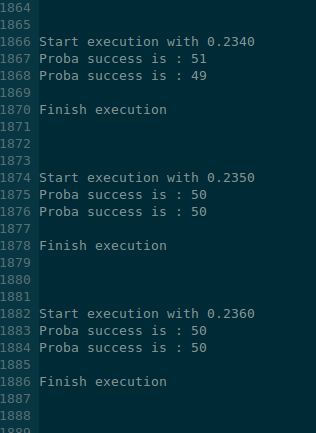
\includegraphics[width=\textwidth]{img/code2.png}
        \label{fig:tiger}
    \end{subfigure}
    ~ %add desired spacing between images, e. g. ~, \quad, \qquad, \hfill etc. 
    %(or a blank line to force the subfigure onto a new line)
    \begin{subfigure}[b]{0.3\textwidth}
        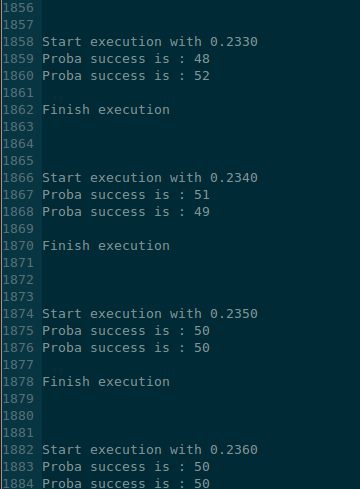
\includegraphics[width=\textwidth]{img/code3.png}
        \label{fig:mouse}
    \end{subfigure}
    \caption{Sorties du programme}\label{fig:animals}
\end{figure}
On remarque alors que lorsque $0,22 < p < 0,23$ les valeurs de succés (matrices égales) et les valeurs d'échecs (matrices différentes) sont presque égales. Elles varient en fonction de la simulation mais de manière générale si p se trouve dans ces valeurs là on commence à avoir un certains nombres d'erreurs non négligeable.
De cette même manière on remarque que pour qu'un code soit optimale (60\% de succés) la valeur de p ne doit pas excéder $0,200$. Lorsque la valeur d'échecs est égales à 60\%, on dit que le décodage n'est pas pertinent, cette condition est atteinte de manière générale lorsque p dépasse la valeur $0,3000$.\\
Le code étudié possède néanmoins une très grande limitation dans le mot qui est passé en paramètre: le nombre d'erreurs trouvés ne pas être égale supérieur à 1! En effet, la méthode pour trouver le bit d'erreur ne prend en compte que le nombre d'erreurs n'est égale à 1. Dans les simulations où le nombre d'erreur était égale à 2 ou plus, le mot décodé n'avait rien à avoir avec le mot d'origine (du fait du mauvais calcul de la position du bit d'erreur).